\chapter{Mitigazione degli attacchi}


\section{Introduzione}

Mitigare gli attacchi DDoS è un problema di più difficile risoluzione rispetto alla sola rilevazione, perché bisogna conoscere maggiori informazioni sulla provenienza del flusso malevolo e il problema dei ``false positive'' è maggiormente sentito: se durante la fase di detection rileviamo un falso positivo e lo notifichiamo all'amministratore di sistema \underline{è un problema relativo} perché sarà lui ad effettuare una successiva analisi prima di intraprendere azioni correttive. Se ci prefiggiamo l'obiettivo di bloccare automaticamente i flussi malevoli dei falsi positivi significherà degradare o impedire la connessione ad utenti legittimi.

\subsection{Ip spoofing}

L'ip spoofing è una tecnica che permette di costruire pacchetti IP con indirizzo IP sorgente modificato con lo scopo di fingersi un altro dispositivo o nascondere la propria identità. È un grande problema di sicurezza delle reti, principalmente perché permette effettuare attacchi DDoS, permettendo di effettuare attacchi come l'amplificazione DNS oppure rendendo più difficile l'identificazione della sorgente dell'attacco nelle altre tipologie.

Un metodo per prevenire o rendere più tracciabili gli attacchi DDoS che lo utilizzano è adottare tecniche in grado di prevenirne il suo utilizzo.

Nello scenario da noi ipotizzato il meccanismo di mitigazione è installato negli edge router nelle sedi aziendali periferiche, in questa posizione possiamo ipotizzare che tutti i pacchetti in transito dalla sotto-rete del distaccamento, verso la sottorete della sede centrale o verso internet, siano stati generati da un host di quella sotto rete. Per questo motivo una soluzione per limitare il problema è impedire al router di effettuare l'inoltro di tutti i pacchetti provenienti da altre sottoreti.
Questa soluzione non elimina completamente il problema dell'ip spoofing, perchè un utente malevolo ha sempre la possibilità di generare traffico utilizzando come indirizzo ip sorgente un qualsiasi indirizzo della stessa subnet.
%todo: cite https://www.cloudflare.com/it-it/learning/ddos/glossary/ip-spoofing/


\paragraph{Bloccare l'ip spoofing}
Per mitigare questo problema abbiamo introdotto una regola iptables nel router \ref{code:iptablesrule}, la quale impedisce l'inoltro di pacchetti provenienti da sottoreti diverse da quella in cui è situato il router.
Iptables è un firewall integrato nel kernel linux basato su netfilter.
% https://wiki.archlinux.org/title/Iptables_(Italiano)#:~:text=Iptables%20%C3%A8%20un%20potente%20firewall,%C3%A8%20usato%20per%20gli%20IPv6.

% todo: la regola è corretta?
\begin{lstlisting}[caption={Esempio di regole iptables}\label{code:iptablesrule}]
    # Accetta i pacchetti della sottorete
    iptables -A INPUT -i internal_interface -s 192.168.0.0/16  -j ACCEPT
    # Fa il drop di tutto ciò che
    # non è esplicitamente accettato
    iptables -P INPUT DROP
\end{lstlisting}


\section{Tool utilizzati}

Per mitigare un attacco bisogna conoscere un maggior numero di informazioni in forma non aggregata riguardanti il traffico, per questo motivo utilizziamo ulteriori tool per la raccolta dei dati non aggregati relativi ai flussi in transito attraverso un'interfaccia del router.

\subsection{Netflow}

Netflow è un software introdotto inizialmente nei router Cisco nel 1996, successivamente è stato creata un'estensione standardizzata dall'IETF, chiamata IPFIX. Netflow è uno dei tool di monitoring più famosi e permette di monitorare e registare informazioni riguardo i flussi che attraversano una determinata interfaccia.
% todo: tabella con features raccolete da netflow

% \begin{center}
%     \begin{tabular}{c c c c c}
%         IN\_BYTES & IN\_PKTS & FLOWS & PROTOCOL & SRC\_TOS \\ TCP\_FLAGS  &  L4\_SRC\_PORT & IPV4\_SRC\_ADDR & SRC\_MASK INPUT\_SNMP \\ L4\_DST\_PORT & IPV4\_DST\_ADDR



%     \end{tabular}
% \end{center}

Poichè non è possibile estendere le features di netflow e quelle esistenti non rispecchiano completamente i nostri interessi abbiamo deciso di progettare il nostro agent utilizzando altre soluzioni.
% todo: le features di netflow le posso modificare?

\subsection{Modulo Kernel}

Nella sezione \ref{section:our_tool} è stata accennata la possibiltà di raccogliere dati con maggiore granularità tramite l'utilizzo di un modulo kernel scritto appositamente.

Nella caso in cui si vogliano aggiungere dei software per collezionare dati maggiormente granulari bisogna intervenire lato kernel, perché in userspace non esistono meccanismi efficienti per analizzare tutti i pacchetti in transito su un'interfaccia. Di conseguenza per aggiungere delle funzioni al kernel Linux esistono solitamente tre soluzioni: la prima è quella di fare aggiungere il codice ufficialmente al suo interno, questa soluzione è la più complicata: sono necessarie le giuste motivazioni per convincere i maintainers ad adottare quella soluzione e inoltre passeranno anni prima della distribuzione in distribuzioni stabili. La seconda è quella di creare un modulo kernel personalizzato, i moduli kernel sono una porzione di codice compilato che possono essere inseriti nel kernel a run-time. Questo metodo è sicuramente più rapido, ma potrebbe portare a vulnerabilità, problemi di compatibilità all'aggiornamento del kernel e rischi di deadlock per l'intero sistema. La terza possibilità è l'uso di eBPF, che esploreremo successivamente.
%TODO: Cercare articolo dove parla del confronto modulo kernel, modulo nativo, ebpf

La prima versione del nostro software è stata sviluppata scrivendo un modulo kernel che utilizzava netfilter. Questa soluzione è la strada tradizionalmente usata nel mondo Linux e in Tiesse per l'implementazione delle proprie personalizzazioni nei prodotti.
Netfilter è un componente di tutte le moderne distribuzioni Linux, che permette di intercettare e manipolare pacchetti in transito dal router, usato nel kernel permette di registrare delle callback, eseguite alla ricezione di ogni pacchetto su un determinato punto d'aggancio.
Per la scrittura del modulo siamo partiti dalla compilazione del codice sorgente del kernel del router. successivamente è stato scritto un programma in linguaggio C, che sfruttando netfilter aggancia ad un hook, più in particolare ``NF\_INET\_POST\_ROUTING'', una funzione da eseguire alla ricezione di ogni pacchetto, la quale incrementa dei contatori di un vettore.
Terminata la scrittura, il modulo deve essere compilato, nel nostro caso cross compilato per architecture ``arm64''. La compilazione genera un file con estensione .ko. Dopo averlo copiato sul router, per renderlo attivo, bisognerà caricarlo dinamicamente nel kernel del router tramite il comando ``insmod [nome\_modulo].ko''.

Inoltre in userspace è stato scritto un plugin per collectd, il quale ogni volta che necessita dei dati effettua una lettura su un ``process file system'' (procfs), uno pseudo-filesystem usato per accedere alle informazioni fornite dai processi kernel, tramite il quale il nostro modulo kernel ritorna un JSON con il nome della metrica presa in considerazione e il valore.

Questa soluzione, nonostante fosse la soluzione da sempre usata in azienda, presenta alcuni problemi come la maggior difficoltà di comunicazione tra user-space e kernel-space, la mancanza di strutture dati già esistenti e soprattutto un problema in questo modulo kernel rischiava di portare ad un completo malfunzionamento dell'intero router, per questa ragione abbiamo deciso di adottare una soluzione più moderna.

\begin{figure}[hbtp]
    \label{fig:netfilter}
    \begin{center}
        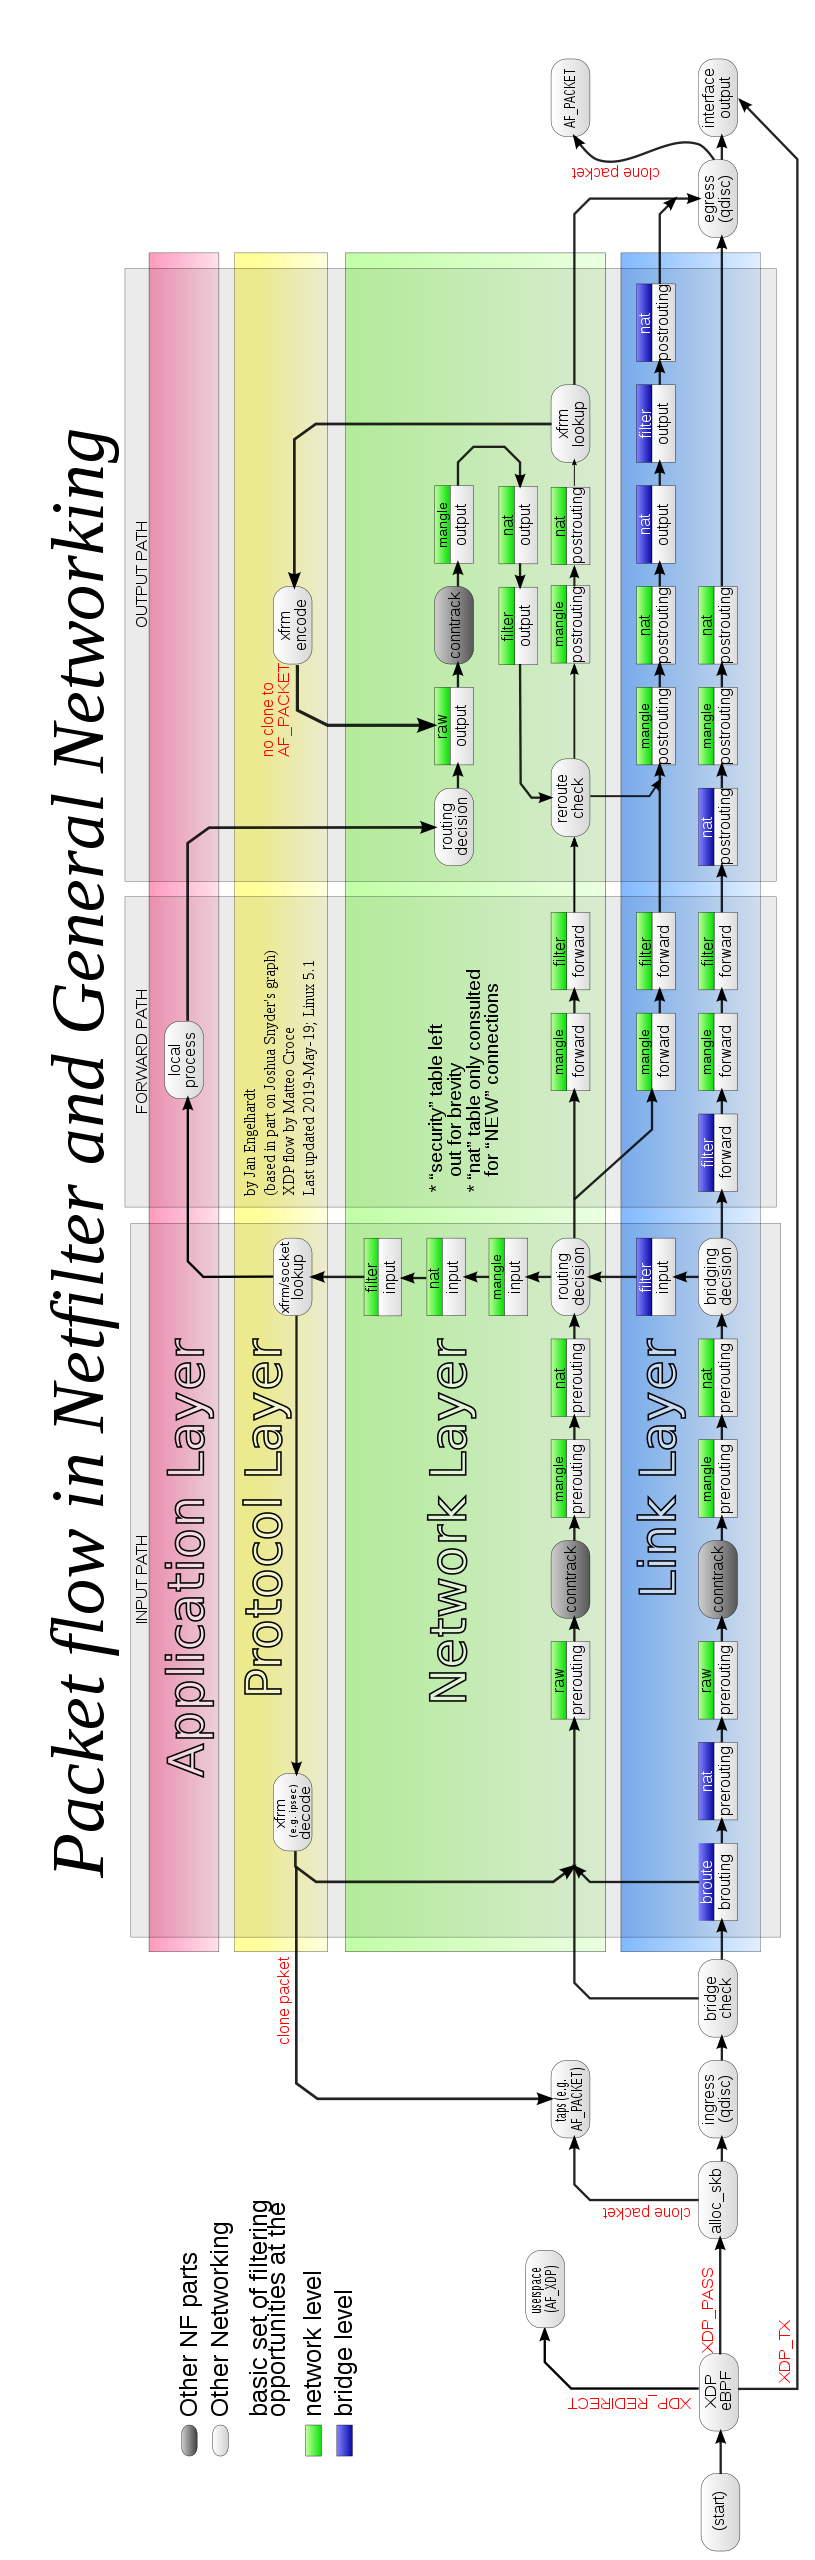
\includegraphics[height=570pt]{images/mitigazione/netfilter.png}
    \end{center}

    \caption{Flusso dei pacchetti in Netfilter \cite{netfilter_img}.}
    \centering
\end{figure}  

\subsection{Berkley Packet Filter (BPF)}

Il Berkley Packet Filter (BPF) è una tecnologia introdotta nel kernel di alcuni sistemi operativi, tra cui il kernel Linux, su cui è stata introdotta nel 1997 a partire dalla versione 2.1.75. BPF consiste in una macchina virtuale, con una virtual cpu special purpose, integrata nel kernel, che permette il filtraggio e l'analisi dei pacchetti in transito su un'interfaccia.
È una soluzione che permette di eseguire un bytecode in maniera sicura nello spazio kernel utilizzando una sandbox ed eliminando l'overhead delle system call e del context switching tra kernel e user. 
Per effettuare il filtering tramite BPF deve essere generato del codice in un particolare assembly in grado di funzionare sulla CPU virtuale, che verrà richiamato alla ricezione di ogni pacchetto sull'interfaccia determinata (event driven). 
Un esempio del suo utilizzo è tcpdump che sfrutta BPF per effettuare il filtraggio in maniera efficiente. L'esempio di bytecode \ref{code:esempiobpf} permette di filtrare i pacchetti IPV4, per farlo verifica se l'ethertype è uguale a 0x800 \cite{risso_ebpf}.

%todo: cite https://drive.google.com/file/d/14dRWGwAJKBqB1N6-NOBHUxoeOILPYQjN/view
% https://docs.cilium.io/en/stable/bpf/

\begin{lstlisting}[caption={Esempio delle istruzioni per il filtering dei pacchetti IP in BPF assembly}\label{code:esempiobpf}]
user@linux$ tcpdump -d ip
(000) ldh [12]
(001) jeq #0 x800 jt 2 jf 3
(002) ret #96
(003) ret #0
\end{lstlisting}

\subsection{extended Berkeley Packet Filter (eBPF)}
% https://docs.cilium.io/en/stable/bpf/

La extended Berkeley Packet Filter è una versione che estende la versione originale ed è stata introdotta nella versione 3.18 del kernel Linux, ai giorni nostri la versione originale è completamente obsoleta e anche il codice scritto per la vecchia versione, per esempio tcpdump, viene tradotto trasparentemente per la nuova \cite{cilium_ebpf}.

\begin{figure}[]
    \label{fig:ebpf}
    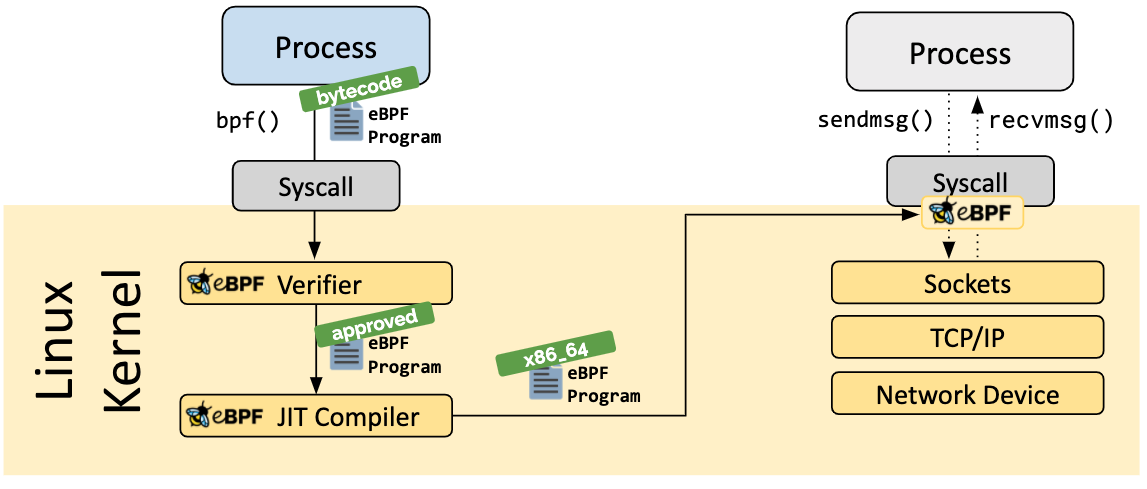
\includegraphics[width=\hsize]{images/mitigazione/ebpf_architecture.png}
    \caption{Architettura eBPF \cite{ebpf.io}.}
    \centering
\end{figure}

Prima che il bytecode sia caricato nel kernel Linux vengono effettuati due passaggi, come si può notare dall'immagine \ref{fig:ebpf}. La prima è la ``Verication'', la quale si occupa di verificare che il programma sia sicuro da eseguire e verifica che: il programma abbia lunghezza limitata, che non ci siano accessi a indirizzi di memoria non validi e che abbia una fine, di conseguenza controlla che non siano presenti cicli infiniti. 
Effettuata la verifica viene eseguita la ``Just-in-Time (JIT) compilation'', la quale traduce il bytecode generico in istruzioni specifiche per la macchina che lo sta eseguendo, questo permette di incrementare le prestazioni e rendere i programmi eBPF efficienti come i moduli kernel compilati nativamente \cite{ebpf.io}.
eBPF inoltre fornisce strumenti utili per lo sviluppo, come le mappe e gli helpers.

Le mappe sono un importante aspetto dei programmi eBPF, esse permettono di memorizzare dati in delle strutture chiave/valore in kernel space, che possono essere condivise con altri programmi eBPF oppure con applicazioni in user space \cite{cilium_ebpf}.

La chiamata di generiche funzioni a livello kernel non è consentita, sia per mantenere la compatibilità del programma non solo con una determinata versione del kernel, per questo motivo sono stati introdotti gli ``helpers'', i quali inoltre permettono l'esecuzione di istruzioni o permettono di eseguire alcuni task non permessi dall'assembly eBPF per motivi di sicurezza.

Un ulteriore caratteristica di eBPF è la possibilità di potere concatenare l'esecuzione dei programmi, chiamandoli a cascata,in maniera simile alla ``execve()'', durante l'esecuzione.

I vantaggi di un programma eBPF rispetto alla scrittura di un modulo kernel sono molteplici: permettono l'esecuzione sicura del codice senza la possibilità che vada a corrompere il kernel, non c'è rischio che le nuovi versioni del kernel vadano a interrompere il suo funzionamento e garantisce le stesse prestazioni.

% https://ebpf.io/

\subsection{eXpress Data Path (XDP)}
\begin{figure}[]
    % todo: capire come gestire citazioni imsmagini a livello di copyright
    % https://www.researchgate.net/publication/333998355_Securing_Linux_with_a_Faster_and_Scalable_Iptables
    \label{fig:hooks}
    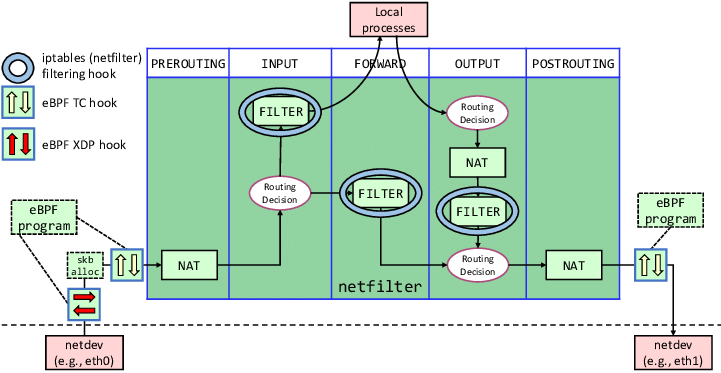
\includegraphics[width=\hsize]{images/mitigazione/hooks.png}
    \caption{Hooks eBPF \cite{risso_ebpf}.}
    \centering
\end{figure}
Il kernel Linux supporta più punti dello stack di rete in cui è possibile agganciare l'esecuzione dei programmi eBPF.
XDP (eXpress Data Path) è un hook ad alte performance che permette di eseguire un programma eBPF al primo punto possibile, questo permette grandi performance, poiché il processamento avviene prima che qualsiasi altra manipolazione possa avvenire. XDP è un punto d'aggancio ideale per il filtering dei pacchetti malevoli o inaspettati e in qualsiasi comune protezione anti DDoS \cite{cilium_xdp}.
Il programma inserito su un hook XDP può compiere cinque azioni possibili:
\begin{itemize}
    \item XDP\_PASS: lascia passare il pacchetto nel normale stack di rete
    \item XDP\_DROP: ignora semplicemente il pacchetto, senza compiere ulteriori azioni
    \item XDP\_TX, restituisce il pacchetto alla stessa interfaccia, normalmente modificato
    \item XDP\_ABORTED: è un valore di ritorno che il programmatore non dovrebbe utilizzare, segnala un che si è verificato un errore nel programma eBPF, per esempio una divisione per zero e contemporaneamente ignora il pacchetto come l'XDP\_DROP
    \item XDP\_REDIRECT: reindirizza il pacchetto verso un'altra scheda di rete, o in user space
\end{itemize}


\subsection{BPF Compiler Collection (BCC)}
 
È un framework che permette la scrittura di programmi python con programmi eBPF incorporati al loro interno. Il framework ha come obiettivo primario i casi in cui eBPF è utilizzata per raccogliere statistiche o compiere azioni in user space al verificarsi di eventi. L'esecuzione del programma eBPF genererà il bytecode che sarà caricato nel kernel \cite{ebpf.io}.
Il programma python potrà comunicare con quello eBPF grazie all'utilizzo delle mappe precedentemente menzionate.

\begin{figure}[]
    \label{fig:bcc}
    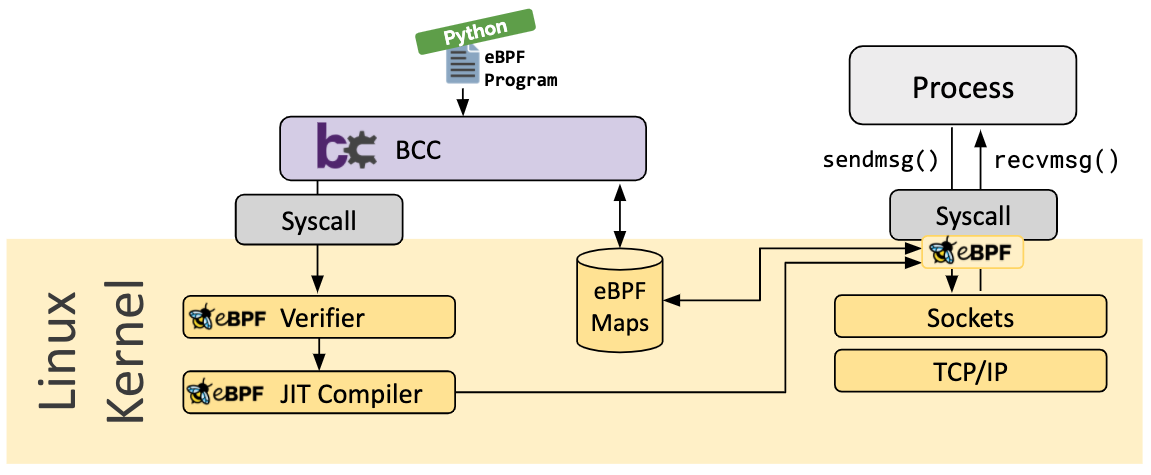
\includegraphics[width=\hsize]{images/mitigazione/bcc.png}
    \caption{Funzionamento di BCC \cite{ebpf.io}.}
    \centering
\end{figure}

\section{Funzionamento}

% Qua posso parlare di due alternative, la prima è riutilizzare il sistema di anomaly detection simile a quello presentato precedentemente elencando tutti i problemi e i vantaggi.

% %todo: citare articoli che usano netflow per rilevare le anomalie

% Il secondo consiste nel raccogliere i dati come prima, e creare un ranking per ogni feature risultata anomala precedentvieneemente e a quel punto blocco i flussi sopra una certa soglia, ma quale?

% Mentre per l'ip spoofing come la gestisco?

Sul server di monitoraggio quando viene rilevata un'anomalia è possibile risalire su quale router sono transitati i dati sospetti, quindi, a questo punto, viene notificato il router della sede periferica responsabile e viene messa in atto la fase di mitigazione.

La fase di mitigazione, raccogliendo dati in forma meno aggregata, è potenzialmente più dispendiosa in termini di risorse, per questo motivo la eseguiamo solo in presenza di un'anomalia sui dati aggregati.

Per metterla in atto per prima cosa dobbiamo raccogliere i dati con minore granularità, per farlo sfruttiamo eBPF, successivamente avviene la fase di decisione in un software o un amministratore di sistema decidono cos'è anomalo e infine sempre tramite eBPF blocchiamo o limitiamo il traffico proveniente da uno o più indirizzi IP.
% todo: come viene notificato?
% todo: accelleratore hardware?

\subsection{Acquisizione dati}

Il funzionamento del sistema di mitigazione da noi ipotizzato si basa sull'utilizzo di un software che sfrutta eBPF, con un'interfaccia in Python 3 generata grazie all'utilizzo di BCC.

Una funzione eBPF scritta per essere eseguita come callback all'arrivo di ogni pacchetto sull'hook XDP di ogni interfaccia ha lo scopo di incrementare dei contatori di pacchetti in una mappa che utilizza come chiave un intero a 64bit generato dall'unione, tramite degli spostamenti bitwise, di ip sorgente, ip destinazione e porta destinazione. L'ip sorgente, per riuscire a mantenere la chiave a soli 64bit, viene troncato a 16 bit: questo permette comunque di identificare l'host sorgente su una rete /16, soluzione aziendale tipica in cui vengono utilizzati i router Tiesse.
Alla ricezione di un pacchetto TCP, UDP e di pacchetti TCP con flag SYN, un RST, FIN oppure pacchetti indirizzati verso una specifica porta, incrementa i relativi contatori. Il software incrementa un contatore anche alla ricezione di ogni pacchetto ICMP, il quale essendo un protocollo incapsulato direttamente in IP non possiede una porta sorgente, per questo motivo la chiave verrà calcolata con il valore di porta destinazione a zero.

% todo: tabella con esempio di dati sui flussi

% todo: trovare nome
\subsection{Fase decisionale - Trovare nome decente}

Grazie alle mappe implementate in eBPF è possibile accedere al loro contenuto anche in userspace. Nel programma in python facciamo accesso alle mappe, leggendo e resettando i contatori e in seguito abbiamo ipotizzato due strade per bloccare le anomalie.

La prima coinvolge un intervento umano, conoscendo quali anomaly score hanno superato le soglie nei dati aggregati, è possibile mostrare una classifica dei flussi con i valori decrescenti relativi alla feature anomala. In questo modo l'operatore potrà, tramite un'interfaccia, bloccare o limitare il flusso per un determinato periodo di tempo. Questa soluzione può essere efficace, perché le anomalie segnalate sui dati aggregati non saranno molte e l'intervento umano permette di bloccare utenti che stanno facendo un uso legittimo della rete, riducendone la loro produttività.

La soluzione alternativa è più complessa e si basa sui principi della precedente fase di anomaly detection.
Per sviluppare questo sistema di mitigazione ci siamo basati nuovamente su una rete neurale, ma a differenza della precedente, la quale lavorava su sequenze temporali di dati, in questo caso il rilevamento delle anomalie viene effettuato sul singolo flusso, con i relativi contatori.

\begin{lstlisting}[language=SQL,caption={Esempio di tabella nel database SQL.}]
create table flows
(
    hostname CHAR(20) not null,
    ip_src INT UNSIGNED not null,
    ip_dst INT UNSIGNED not null,
    port_dst SMALLINT UNSIGNED not null,
    timestamp timestamp not null,
    syn_tx INT UNSIGNED not null,
    fin_tx INT UNSIGNED not null,
    rst_tx INT UNSIGNED not null,
    udp_tx INT UNSIGNED not null,
    tcp_tx INT UNSIGNED not null,
    icmp_tx INT UNSIGNED not null,
    packet_rate_tx INT UNSIGNED not null,
    throughput_tx INT UNSIGNED not null,
    udp_tx_53 INT UNSIGNED not null,
    constraint flows_pk
        primary key (hostname, port_dst,
            ip_src, ip_dst, timestamp)
);
\end{lstlisting}

\subsection{Riconoscimento flussi anomali tramite rete neurale}

Per effettuare il riconoscimento dei flussi anomali senza l'intervento umano abbiamo ipotizzato di utilizzare una rete neurale di autoencoder, che necessita dei dati per effettuare l'allenamento.

Per quanto riguarda la raccolta dei dati da utilizzare per il train, abbiamo previsto una fase in cui le informazioni riguardo i contatori di pacchetti, delle diverse tipologie, per ogni flusso in transito attraverso il router in un determinato periodo di tempo,nel nostro caso 30 secondi, vengono inviate su un database SQL (nel nostro caso abbiamo utilizzato MariaDB).

Raccolta una quantità adeguata di dati, utilizzando il server utilizzato per l'anomaly detection, è possibile effettuare il train della rete neurale, calcolare le soglie e terminare l'acquisizione dei dati e volendo è possibile anche cancellare i dati relativi all'allenamento dal database. I dati necessari per il train possono essere raccolti contemporaneamente da tutte le sedi aziendali, poiché i flussi per singolo utente saranno simili in ogni distaccamento, indipendentemente dalla grandezza di esso.

Nel momento in cui viene rilevata un'anomalia sui dati aggregati, è necessario riavviare la fase di raccolta delle informazioni riguardanti i flussi, seguita dal calcolo degli anomaly score relativi ad ogni flusso. Se il flusso è anomalo essendo a conoscenza dell'ip sorgente è possibile prendere azioni per limitarlo.


\subsection{Bloccare gli attacchi}

Identificati i flussi anomali grazie all'utilizzo di un'ulteriore mappa condivisa con il codice eBPF, dall'interfaccia è possibile comunicare su quali flussi applicare i blocchi oppure su quali applicare delle restrizioni.
Nel nostro esempio abbiamo usato una mappa, tramite la quale è possibile comunicare alla funzione eBPF quali pacchetti bloccare. Volendo sarebbe possibile differenziare i comportamenti in base alla tipologia di attacco, per esempio in caso di SYN flood si potrebbero limitare solo quelli.

Gli attacchi DDoS effettuati utilizzando la tecnica dell'ip spoofing è possibile bloccarli facilmente nel caso in cui l'indirizzo ip sorgente non appartenga alla subnet, ma è ancora possibile effettuare attacchi con gli ip della sottorete.
In questo secondo caso è più difficile identificarli, ma è comunque possibile identificare grandi variazioni nel numero di indirizzi ip che trasmettono e di conseguenza imporre dei limiti a tutta la sottorete.

Bloccare o modificare flussi appartenenti ad applicazioni mission-critical è sempre molto pericoloso da effettuare senza l'intervento umano, quindi potrebbe essere necessario chiedere una conferma all'amministratore di rete.

% todo: come decidiamo le soglie? in caso di intervento umano può decidere lui, in caso di intervento automatico possiamo basarci su


% \section{Test sulle anomalie}
% \subsection{Tool utilizzati}
\section{Risultati}

I risultati ottenuti tramite l'utilizzo del sistema di anomaly detection sui singoli flussi sono molto promettenti, nel caso in cui il traffico sia generato da applicazioni aziendali specifiche è anche più facilmente riconoscibile, ma bisogna valutare attentamente il livello di criticità dell'applicazione, perchè in caso di un errore dovuto ad un utilizzo insolito dell'applicativo c'è il rischio di degradare o interrompere il lavoro di un utente, per questa ragione bisogna valutare caso per caso quale sia la migliore reazione da prendere.

